\chapter{Graph}

Graph merupakan sebuah \textit{Abstract Data Type} (ADT) yang digunakan untuk mengimplementasikan konsep \textit{graph} dan \textit{directed graph} dalam matematika. Dalam matematika sendiri, graph merupakan sebuah representasi dari sekumpulan objek yang saling terhubung. Objek-objek yang ada di dalam graph dikenal dengan nama \textit{vertex}, sedangkan hubungan (penghubung) antar objek tersebut dikenal dengan nama \textit{edge}.

Sebuah graph dapat digunakan untuk merepresentasikan banyak hal dalam dunia nyata. Misalnya, kita dapat merepresentasikan pohon pengetahuan dalam sebuah graph seperti yang nampak pada gambar~\ref{fig:knowledge-tree}. Peta juga kerap kali direpresentasikan sebagai graph, dengan titik-titik pergerakan sebagai vertex-nya, dan jalur antar titik sebagai edge-nya (lihat gambar~\ref{fig:map-graph}).

\begin{figure}
    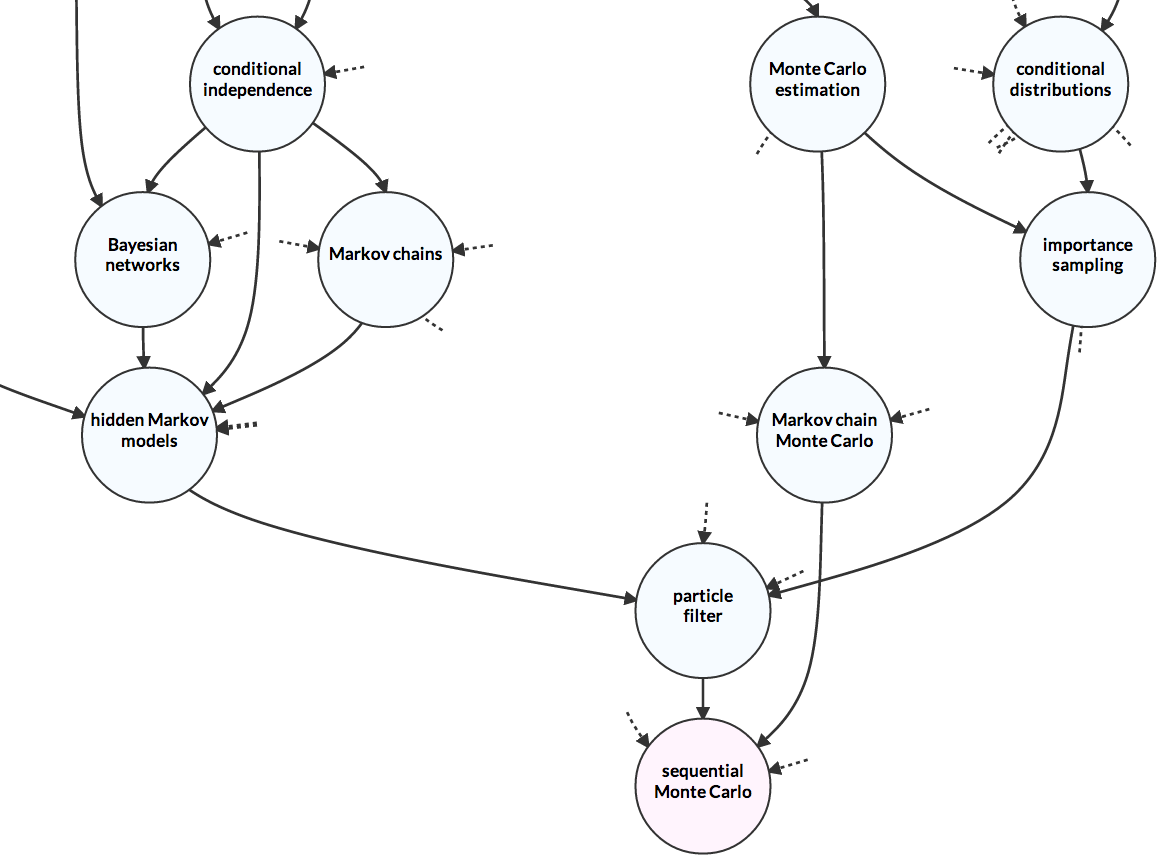
\includegraphics[width=\textwidth,keepaspectratio]{fig/KnowledgeTree.png}%
	\caption{Pohon Pengetahuan}%
	\label{fig:knowledge-tree}%
\end{figure}

\begin{figure}
    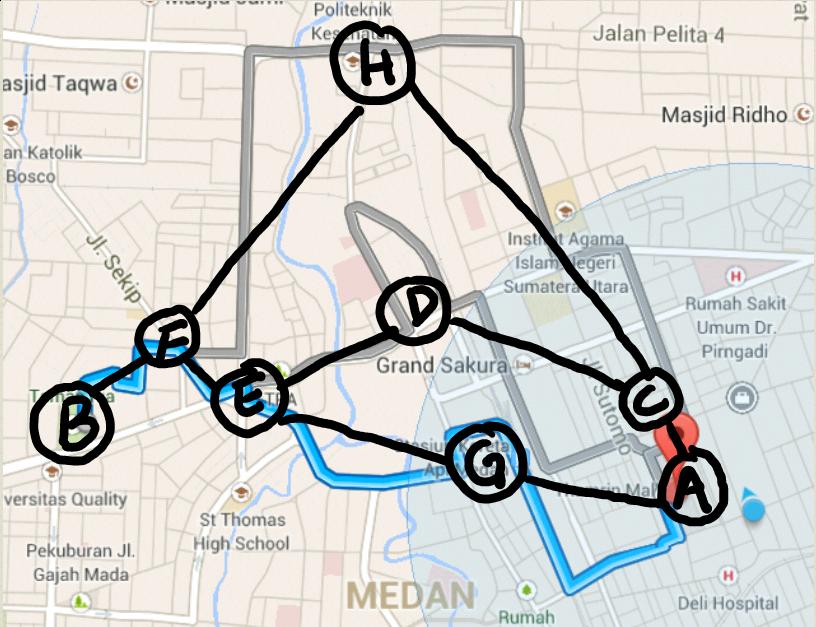
\includegraphics[width=\textwidth,keepaspectratio]{fig/DirectedGraphMap.png}%
	\caption{Peta dengan Graph}%
	\label{fig:map-graph}%
\end{figure}

Terdapat sangat banyak jenis dan definisi dari graph, yang masing-masing memiliki kegunaan spesifik dan kelebihan serta kekurangan tersendiri. Pada bagian ini kita hanya akan membahas satu jenis graph, yaitu graph tidak berarah yang berlabel. Untuk mengetahui lebih lanjut mengenai detil dari berbagai jenis graph serta kelebihan dan kekurangannya, silahkan baca buku atau modul tentang struktur data terkait.

Graph tidak berarah berlabel yang kita gunakan didefinisikan sebagai berikut:

\begin{itemize}
    \item Sebuah graph didefinisikan sebagai $G = (V, E)$.
    \item $V$ merupakan sekumpulan vertex.
    \item $E$ merupakan sekumpulan edge.
    \item $E = (V1, V2, v)$ di mana $V1$ dan $V2$ adalah dua buah vertex yang terhubung dan $v$ adalah label (bobot; jarak) dari kedua vertex tersebut.
    \item Dua buah vertex yang saling berdampingan membentuk sebuah edge dapat dihubungkand engan simbol $~$, sehingga $u ~ v$ dapat dibaca sebagai vertex $u$ dan $v$ yang berdampingan (memiliki edge).
\end{itemize}

Definisi graph yang kita gunakan tidak terlalu jauh berbeda dengan yang digunakan pada teori graph dalam matematika pada umumnya. Tetapi ingat bahwa definisi ini seringkali dimodifikasi sesuai dengan kebutuhan dan tujuan dari algoritma yang menggunakan graph tersebut. Misalnya, representasi dan definisi dari sebuah graph yang digunakan untuk menyelesaikan permasalahan pemetaan seperti mencari jalur terpendek akan berbeda dengan representasi untuk menyelesaikan masalah deteksi bahasa. Begitupun, algoritma-algoritma dasar yang sama dapat kita immplementasikan pada representasi graph yang berbeda ini (misalnya: algoritma untuk pencarian jalur terpendek). Perbedaan hanya akan ditemukan pada detil implementasi nantinya.

Untuk memperjelas pengertian tentang representasi graph yang berbeda, kita akan melihat beberapa jenis cara merepresentasikan graph yang umum digunakan.

\section{Representasi Graph}

Sebagai sebuah struktur data tingkat tinggi, kita umumnya akan membangun graph dengan menggabungkan beberapa struktur data sederhana seperti array, struktur, atau objek. Beberapa struktur data sederhana ini kemudian diintegrasikan dengan aturan tertentu agar dapat direpresentasikan sebagai graph. Secara umum terdapat tiga metode untuk merepresentasikan graph dari struktur-struktur sederhana seperti ini, yaitu:

\begin{description}
    \item[Adjacency List] \hfill \\
        Pada adjacency list, vertex direpresentasikan sebagai sebuah objek khusus (mulai dari yang sederhana seperti string sampai objek buatan sendiri). Vertex kemudian disimpan di dalam sebuah list atau array, dan setiap vertex menyimpan list atau array dari vertex yang berdampingan.
    \item[Adjacency Matrix] \hfill \\
        Pada adjacency matrix, kita menyimpan data graph di dalam sebuah matriks, dengan bagian baris sebagai vertex asal dan bagian kolom sebagai vertex tujuan. Isi dari matriks sendiri adalah jumlah edge yang menghubungkan kedua vertex (baris dan kolom). Data dari semua vertex dan edge sendiri harus di luar matriks.
    \item[Incidence Matrix] \hfill \\
        Pada incidence matrix, graph direpresentasikan dalam matriks dua dimensi, dengan baris matriks sebagai vertex dan kolom matriks sebagai edge. Nilai dari matriks mengindikasikan keterhubungan (\textit{incidence}) antara vertex dengan edge.
\end{description}

Untuk melihat detil yang dijabarkan, mari kita lihat masing-masing representasi ini dengan lebih mendalam.

\subsection{Graph dengan Adjacency List}

Seperti yang telah dijelaskan sebelumnya, pada representasi graph dengan adjacency list, kita terlebih dahulu menyimpan seluruh vertex ke dalam sebuah list. Semua vertex ini kemudian menyimpan sebuah list lagi, yang berisi vertex lain yang berdekatan dengannya. Gambar~\ref{fig:graph-adj-list} mengilustrasikan graph yang direpresentasikan dengan adjacent list.

\begin{figure}[h!]
    \centering
    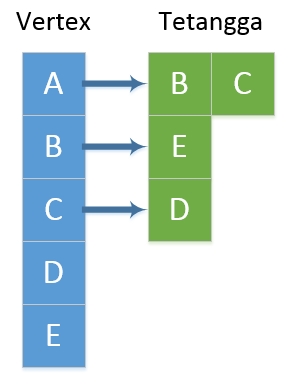
\includegraphics[width=.3\textwidth,keepaspectratio]{fig/Graph-AdjacencyList.png}%
	\caption{Graph dengan Adjacency List}%
	\label{fig:graph-adj-list}%
\end{figure}

\FloatBarrier

Untuk membuat graph dengan adjacency list, kita dapat mulai dengan mentukan objek vertex terlebih dahulu. Dengan asumsi kita merepresentasikan objek vertex sebagai sebuah string sederhana (yang tidak mengandung nilai), kita dapat menyimpan sebuah graph seperti gambar~\ref{fig:graph-adj-list} dengan menggunakan struktur data dictionary sederhana seperti pada algoritma~\ref{algo:graph-dict}.

\lstinputlisting[language=Python, 
                 label={algo:graph-dict},
                 caption=Sebuah Graph dengan Dictionary
                ]
                {code/14-graph-dict.py}

Algoritma~\ref{algo:graph-dict} memperlihatkan bagaimana kita dapat memanfaatkan dictionary dengan aturan tertentu untuk merepresentasikan graph. Adapun aturan yang kita gunakan yaitu:

\begin{itemize}
    \item Kunci dictionary merepresentasikan vertex dari graph.
    \item Setiap kunci (vertex) berisi list.
    \item List yang dimiliki oleh setiap vertex berisi daftar vertex lain yang berdekatan dengannya.
\end{itemize}

Pembentukan graph seperti ini merupakan salah satu implementasi yang paling sederhana, dan sangat mudah diimplementasikan. Jika ingin menghubungkan $v1$ ke $v2$ dan membuat edge $v1 ~ v2$, kita cukup menambahkan $v2$ ke dalam list yang ada pada $v1$. Penyimpanan nilai vertex juga dapat dilakukan dengan menggunakan dictionary jika kita ingin menambahkan nilai di dalam edge. Algoritma~\ref{algo:graph-dict-dict} menunjukkan contoh implementasi jika ingin menyimpan graph berlabel.

\lstinputlisting[language=Python, 
                 label={algo:graph-dict-dict},
                 caption=Graph dengan Adjacency List yang Berlabel
                ]
                {code/15-graph-dict-dict.py}

Pada represenatsi graph dengan adjacency list, kita hanya menyimpan vertex yang berdekatan secara langsung dengan vertex utama saja. Perhatikan bagaimana pada algoritma~\ref{algo:graph-dict-dict} vertex $D$ dan $E$ hanya mengandung list kosong, karena kedua vertex ini tidak memiliki vertex lain didekatnya. Dengan tidak menyimpan data yang tidak diperlukan seperti ini tentunya adjacency list menggunakan memori secara optimal (tidak menyimpan data yang tidakdiperlukan).

Kekurangan utama dari representasi graph dengan adjacency list seperti ini sendiri yaitu untuk pengecekan apakah dua buah vertex saling berdekatan. Karena kita tidak dapat langsung melakukan pengecekan baris-kolom seperti pada adjacency matrix, operasi ini otomatis akan harus dilakukan dengan megecek satu per satu kunci di dalam vertex, yang akhirnya akan memberikan operasi $O(n)$, yang dapat dikatakan lambat dibandingkan dengan operasi $O(1)$ pada adjacency matrix.

\subsection{Graph dengan Adjacency Matrix}

Jika pada representasi graph dengan adjacency list kita menyimpan data di dalam dictionary dan list, pada adjacency matrix kita akan menyimpan data ke dalam sebuah matriks. Seperti matriks pada umumnya, graph dapat diimplementasikan dalam array dua dimensi. Untuk lebih mempermudah pengertian, gambar~\ref{fig:graph-adj-matrix} memperlihatkan contoh graph beserta dengan adjacency matrix-nya.

\begin{figure}
    \centering
    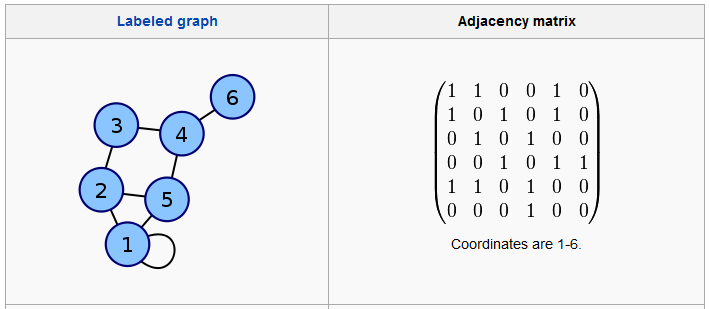
\includegraphics[width=\textwidth,keepaspectratio]{fig/Graph-AdjacencyMatrix.png}%
	\caption{Graph dengan Adjacency Matrix}%
	\label{fig:graph-adj-matrix}%
\end{figure}

Seperti yang telah dijelaskan sebelumnya, setiap baris pada matriks yang ada di gambar~\ref{fig:graph-adj-matrix} merepresentasikan vertex dari grafik. Hal ini berarti baris pertama merepresentasikan vertex $1$, baris kedua mewakilkan vertex $2$, dst. Kolom dari matriks sendiri merepresentasikan semua vertex lain yang ada (kolom 1 untuk vertex $1$, kolom 2 untuk vertex $2$, dst). Nilai dari matriks(baris, kolom) sendiri akan berisi 1 jika vertex baris-kolom memiliki hubungan, dan bernilai 0 jika tidak.

Karena setiap vertex harus disimpan dua kali (dalam baris dan kolom matriks), maka matriks yang dihasilkan oleh adjacency matrix akan selalu berukuran $n \times n$. Hal ini berarti penggunaan memori dari adjacency matrix secara otomatis akan lebih besar dibandingkan adjacency list. Sifat penyimpanan vertex di baris dan kolom ini juga menyebabkan penambahan dan penghapusan vertex menjadi lebih lambat karena setiap kali terjadi penambahan dan penghapusan kita harus mengubah ukuran matriks (yang umumnya adalah operasi $O(n^2)$). Untungnya, penambahan dan pengurangan edge tidak terpengaruh, karena penambahan dan pengurangan edge hanya akan memerlukan operasi perubahan nilai matriks.

Berkebalikan dengan representasi adjacency list, adjacency matrix justru mudah dalam melakukan operasi pengecekan apakah $v1$ dan $v2$ saling berdekatan. Karena matriks yang umumnya direpresentasikan dalam bentuk array dua dimensi, pengecekan cukup dilakukan dengan mengakses indeks array dari matriks dan melihat apakah nilai berisi 1 dan 0. Hal ini berarti kompleksitas yang dibutuhkan untuk operasi ini hanya $O(1)$, karena operasi akses nilai matriks yang bersifat konstan.

\subsection{Graph dengan Incidence Matrix}

Representasi graph dengan incidence matrix tidak jauh berbeda dengan adjacent matrix. Kita tetap merepresentasikan graph dengan matriks, dengan sedikit perbedaan: kolom matriks sekarang merepresentasikan \textit{edge}, bukan lagi \textit{vertex}. Gambar~\ref{fig:graph-incidence-matrix} memperlihatkan hubungan baris-kolom ini.

\begin{figure}
    \centering
    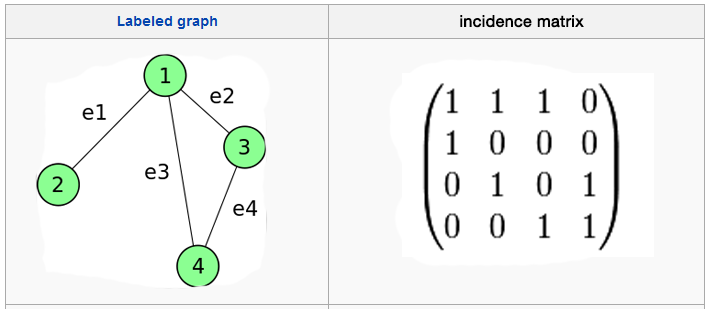
\includegraphics[width=\textwidth,keepaspectratio]{fig/Graph-IncidenceMatrix.png}%
	\caption{Graph dengan Incidence Matrix}%
	\label{fig:graph-incidence-matrix}%
\end{figure}

Meskipun mirip dengan adjacency matrix, graph dengan incidence matrix memiliki sebuah kekurangan besar dibandingkan dengan adjacency matrix: operasi penambahan dan pengurangan edge akan memiliki kompleksitas $O(V \times E)$, karena penambahan dan pengurangan edge akan mengharuskan kita mengubah matriks. Operasi-operasi lain seperti penambahan dan pengurangan vertex memiliki kompleksitas yang mirip dengan adjacency matrix, yaitu $O(V \times E)$. Perubahan hanya terjadi pada faktor pengali, yang awalnya adalah vertex pada adjacency matrix, diganti menjadi edge pada incidence matrix.

\section{Operasi Umum Graph}

Terdapat beberapa operasi umum yang dapat dilakukan terhadap graph, yaitu:

\begin{enumerate}
    \item Penambahan Vertex baru
    \item Penambahan Edge baru
    \item Penghapusan Vertex
    \item Penghapusan Edge
    \item Pengecekan apakah dua buah vertex terhubung
\end{enumerate}

Kompleksitas dari masing-masing operasi sendiri berbeda-beda, tergantung dari cara representasi graph yang kita gunakan. Untuk mempermudah pengertian, kita akan langsung mencoba mengimplementasikan graph dengan adjacency list, dan melihat bagaimana cara implementasi kelima operasi ini.

\section{Contoh Implementasi Graph: Adjacency List}

Implementasi graph dapat dimulai dari pembuatan sebuah kelas untuk graph seperti yang dapat dilihat pada algoritma~\ref{algo:migraph-class}.

\lstinputlisting[language=Python, 
                 firstline=1,
                 lastline=1,
                 label={algo:migraph-class},
                 caption=Definisi Kelas MiGraph
                ]
                {code/migraph.py}

Struktur graph sendiri disimpan ke dalam sebuah variabel privat, yang adalah sebuah \textit{dictionary}. Pembuatan struktur internal graph ini dibuat pada saat objek dibuat. Pengguna juga dapat memberikan graph sesuai dengan struktur internal, seperti yang tampak pada algoritma~\ref{algo:migraph-constructor}.

\lstinputlisting[language=Python, 
                 firstline=16,
                 lastline=17,
                 label={algo:migraph-constructor},
                 caption=Definisi Constructor MiGraph
                ]
                {code/migraph.py}

Pengambilan seluruh vertex dan edge yang ada dapat dilakukan dengan cukup gamblang: hanya mengubah kunci dictionary menjadi list untuk vertex, dan menelusuri isi value dari dictionary untuk edges. Algoritma~\ref{algo:migraph-vertices-edges} menunjukkan cara kerja dari bagian pengambilan seluruh vertex dan edge.

\lstinputlisting[language=Python, 
                 firstline=19,
                 lastline=30,
                 label={algo:migraph-vertices-edges},
                 caption=Pengambilan Seluruh Vertex dan Edge
                ]
                {code/migraph.py}

Karena cara penyimpanan adjacent list yang menyimpan semua vertex tetangga di dalam key dictionary, kita dapat mengecek apakah sebuah vertex bertetangga dengan vertex lain dengan sangat mudah. Algoritma~\ref{algo:migraph-is-adjacent} memperlihatkan implementasi fungsi untuk pengecekan apakah vertex bertetangga dengan vertex lainnya.

\lstinputlisting[language=Python, 
                 firstline=32,
                 lastline=33,
                 label={algo:migraph-is-adjacent},
                 caption=Cek Apakah $v1$ dan $v2$ Bertetangga
                ]
                {code/migraph.py}

Penambahan vertex dan edge juga dapat dilakukan dengan sangat sederhana: tambahkan nilai baru di dalam dictionary atau list sesuai dengan kebutuhan. Algoritma~\ref{algo:migraph-add-vertex-edge} memperlihatkan cara implementasi fungsi penambahan vertex dan edge.

\lstinputlisting[language=Python, 
                 firstline=35,
                 lastline=56,
                 label={algo:migraph-add-vertex-edge},
                 caption=Penambahan Vertex dan Edge
                ]
                {code/migraph.py}

Pengambilan vertex yang ada di sekitar vertex sendiri dilakukan dengan cara yang sama dengan pengambilan vertex: hanya mengubah key menjadi list. Algoritma~\ref{algo:migraph-get-neighbour} menunjukkan langkah yang digunakan.

\lstinputlisting[language=Python, 
                 firstline=58,
                 lastline=68,
                 label={algo:migraph-get-neighbour},
                 caption=Pengambilan Vertex Sekitar
                ]
                {code/migraph.py}

Penghapusan vertex maupun edge dilakukan dengan cara yang sama dengan penambahan dan pengambilan nilai vertex, yaitu sesuai dengan semantik python. Algoritma~\ref{algo:migraph-remove-vertex-edge} menunjukkan langkah yang digunakan.

\lstinputlisting[language=Python, 
                 firstline=70,
                 lastline=78,
                 label={algo:migraph-remove-vertex-edge},
                 caption=Penghapusan Vertex dan Edge
                ]
                {code/migraph.py}

\section{Akhir Kata}

Pada bagian ini kita telah mempelajari berbagai representasi dari graph, kelebihan dan kekurangan dari masing-masing representasi tersebut, serta bagaimana mengimplementasikan salah satu dari representasi tersebut. Pengetahuan yang kita dapatkan pada bagian ini akan diguankan untuk bagian selanjutnya, yaitu algoritma penelusuran graph.
